% Nallino, Part II p. 240: the equation of the centre, redrawn from the print at the size of the print. The
% coordinates are those of a 400 dpi render of the figure (crop from x 100 pt, y 279 pt of the master page; y downward).
% ABD is the ecliptic about the Earth E, GHK the deferent; E' is the centre of the equant, M that of the deferent
% (the dashed lines meet a little above the centre of the drawn circle, as on the print), H the centre of the
% epicycle; ZHE' and XHE are the lines from the equant and from the Earth, E'N (dashed) the prolongation of ZHE',
% EN and MS the perpendiculars on it.
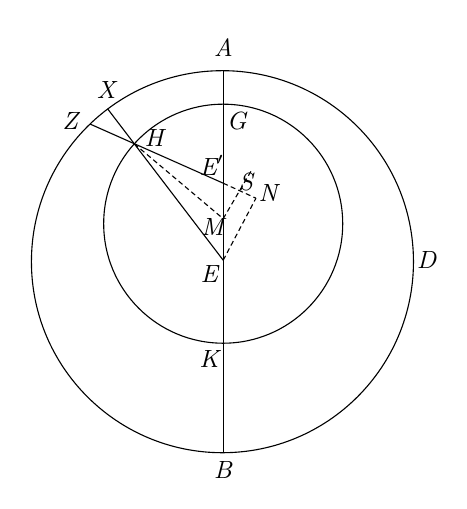
\begin{tikzpicture}[x=0.0635mm,y=-0.0635mm,line width=0.4pt,every node/.style={font=\itshape\small,inner sep=1pt}]
\path (0,20);
\coordinate (Ep) at (391,331);
\coordinate (M) at (391,402);
\coordinate (E) at (391,485);
\coordinate (H) at (213,252);
\coordinate (Z) at (124.7,212.7);
\coordinate (X) at (160,182.5);
\coordinate (S) at (424,347.5);
\coordinate (N) at (456.5,361);
\draw (389.5,488) circle[radius=382];
\draw (391,412) circle[radius=239];
\draw (391,106) -- (391,871);
\draw (Z) -- (Ep);
\draw (X) -- (E);
\begin{scope}[dash pattern=on 1.8pt off 1.2pt]
\draw (Ep) -- (N);
\draw (H) -- (M);
\draw (M) -- (449,303);
\draw (E) -- (N);
\end{scope}
\node at (391.5,61) {A};
\node at (418,206) {G};
\node at (85,206) {Z};
\node at (157,144) {X};
\node at (253,240) {H};
\node at (361,295) {E\rlap{$'$}};
\node at (436,329) {S};
\node at (481,351) {N};
\node at (370,419) {M};
\node at (363,512) {E};
\node at (363,682.5) {K};
\node at (390.5,904) {B};
\node at (797.5,485) {D};
\end{tikzpicture}
